\documentclass[aspectratio=169,10pt,t]{beamer}
% \usetheme[
% %%% options passed to the outer theme
% %    progressstyle=fixedCircCnt,   %either fixedCircCnt, movCircCnt, or corner
% %    rotationcw,          % change the rotation direction from counter-clockwise to clockwise
% %    shownavsym          % show the navigation symbols
%   ]{SDUsimple}
\usepackage{SDUtheme/beamerthemeSDUsimple}
% If you want to change the colors of the various elements in the theme, edit and uncomment the following lines
% Change the bar and sidebar colors:
%\setbeamercolor{SDUsimple}{fg=red!20,bg=red}
%\setbeamercolor{sidebar}{bg=red!20}
% Change the color of the structural elements:
%\setbeamercolor{structure}{fg=red}
% Change the frame title text color:
%\setbeamercolor{frametitle}{fg=blue}
% Change the normal text color background:
%\setbeamercolor{normal text}{fg=black,bg=gray!10}
% ... and you can of course change a lot more - see the beamer user manual.
\usepackage{color}
\usepackage{float}
\usepackage{dsfont}                         % Enables double stroke fonts
\usepackage{bm}
\usepackage[utf8]{inputenc}
\usepackage[english]{babel}
\usepackage[T1]{fontenc}
\usepackage{booktabs}
\usepackage{minted}
\setminted{linenos=true,breaklines=true,obeytabs=true,tabsize=2}
\usepackage{import}
\newcommand{\includesvg}[2][./]{%
    \immediate\write18{inkscape #1#2.svg --export-latex -D --export-filename=#1#2.pdf }
\import{#1}{#2.pdf_tex}
}
% Or whatever. Note that the encoding and the font should match. If T1
% does not look nice, try deleting the line with the fontenc.
\usepackage{helvet}
\usefonttheme{professionalfonts}

\newtheorem{algorithm}{Algorithm}
%\newtheorem{problem}{Problem}
\newtheorem{proposition}{Proposition}
% colored hyperlinks
\newcommand{\chref}[2]{%
  \href{#1}{{\usebeamercolor[bg]{SDUsimple}#2}}%
}

\title{HTTP, PHP, Sessions and Cookies}
\subtitle{Backend stuff ish}
%\date{\today}
\date{ }

\author{
  \textbf{ITI-F20}
}

% - Give the names in the same order as they appear in the paper.
% - Use the \inst{?} command only if the authors have different
%   affiliation. See the beamer manual for an example

\institute[
%  {\includegraphics[scale=0.2]{SDU_segl}}\\ %insert a company, department or university logo
  SDU Robotics\\
  The Maersk Mc-Kinney Moller Institute\\
  University of Southern Denmark
] % optional - is placed in the bottom of the sidebar on every slide
{% is placed on the bottom of the title page
  SDU Robotics\\
  The Maersk Mc-Kinney Moller Institute\\
  University of Southern Denmark

  %there must be an empty line above this line - otherwise some unwanted space is added between the university and the country (I do not know why;( )
}

% specify a logo on the titlepage (you can specify additional logos an include them in
% institute command below
\pgfdeclareimage[height=0.5cm]{titlepagelogo}{SDUgraphics/SDU_logo_new} % placed on the title page
%\pgfdeclareimage[height=1.5cm]{titlepagelogo2}{SDUgraphics/SDU_logo_new} % placed on the title page
\titlegraphic{% is placed on the bottom of the title page
  \pgfuseimage{titlepagelogo}
%  \hspace{1cm}\pgfuseimage{titlepagelogo2}
}

\begin{document}
% the titlepage
{\SDUwavesbg%
\begin{frame}[plain,noframenumbering] % the plain option removes the header from the title page
  \titlepage
\end{frame}}
%%%%%%%%%%%%%%%%

% TOC
\begin{frame}{Agenda}{\vphantom{(y}}
	\begin{itemize}
		\item HTTP verbs
		\item Sessions - Cookies
		\item Superglobals
		\item Cross Site Scripting
		\item HTTPS vs HTTP
	\end{itemize}
\end{frame}
%%%%%%%%%%%%%%%


\begin{frame}[fragile]
	\frametitle{HTTP}
	\framesubtitle{Verbs}
	\begin{itemize}
		\item GET
		\item POST
		\item PUT
		\item DELETE
	\end{itemize}
\end{frame}

\begin{frame}[fragile]
	\frametitle{Session \& Cookies}
	\framesubtitle{Be wary of the cookie monster}
	\vfill
	\begin{figure}
		\centering
		\includesvg[./]{sessionCookie}
	\end{figure}
	\vfill
\end{frame}

\begin{frame}[fragile]
	\frametitle{Superglobals}
	\framesubtitle{Everything is consistent, except when it is not}
	\begin{itemize}
		\item \mintinline{php}{$_SESSION}
		\item \mintinline{php}{$_COOKIES}
		\item \mintinline{php}{$_POST}
		\item \mintinline{php}{$_GET}
	\end{itemize}
	\pause
	\vfill
		\begin{minted}{php}
<?php
if (session_status() == PHP_SESSION_NONE) {
	session_start();
}
		\end{minted}
\end{frame}

\begin{frame}[fragile]
	\frametitle{Cross-Site Scripting}
	\framesubtitle{aka Offroad}
	\begin{figure}[h]
		\centering
		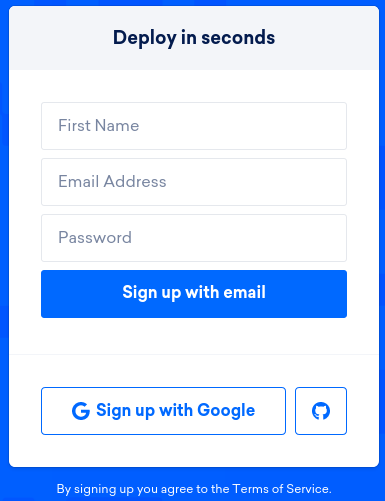
\includegraphics[width=0.3\textwidth]{input.png}
%		\def\svgwidth{0.3\textwidth}
		%\scalebox{0.7}{
		%	\includesvg{input}
		%}
	\end{figure}
	\mintinline{php}{$sanitizedSubject = filter_var ($Subject, FILTER_SANITIZE_SPECIAL_CHARS);}
\end{frame}


\begin{frame}[fragile]
	\frametitle{HTTP vs HTTPS}
	\framesubtitle{Symmetric and Asymmetric}
	\begin{figure}[h]
		\centering
		\def\svgwidth{0.7\textwidth}
		\includesvg[./]{http-vs-https}
	\end{figure}
\footnote{https://www.cloudflare.com/learning/ssl/what-is-ssl/}	
\end{frame}

\end{document}
